
El diseño del hardware de \textit{NodeAlert IoT} adopta un enfoque de diseño por capas, lo que permite una clara separación de funciones y facilita el mantenimiento y la escalabilidad.

\subsection{Nodos IoT Periféricos (Capa de Adquisición)}
Los nodos periféricos están centrados en el microcontrolador ESP32 debido a su capacidad de procesamiento de doble núcleo y conectividad Wi-Fi integrada. Estos nodos son los encargados de interactuar directamente con el entorno físico.

\begin{itemize}
    \item \textbf{Sensores:} Se utilizan sensores de respuesta rápida para variables críticas. Según \citet{boylestad2009}, el tiempo de recuperación y la sensibilidad de los dispositivos semiconductores son vitales para la precisión. Se integran:
    \begin{itemize}
        \item \textbf{DHT22:} Para humedad y temperatura, con comunicación digital.
        \item \textbf{MQ-9:} Sensor electroquímico para detección de monóxido de carbono y gases inflamables.
        \item \textbf{KY-026:} Sensor infrarrojo para detección de espectro de llama.
    \end{itemize}
    \item \textbf{Actuador (Buzzer):} Cada nodo cuenta con un buzzer activo conectado al GPIO2 a través de un transistor 2N2222 con resistencia de base de 1k$\Omega$, necesario porque el buzzer consume entre 50 y 100mA, superando la corriente máxima de 40mA del GPIO. El buzzer reproduce patrones diferenciados seg\'un la severidad de la alerta (WARNING, CRITICAL, EMERGENCY).
\end{itemize}

\subsection{Servidor (Raspberry Pi)}
La infraestructura central reside en una \textbf{Raspberry Pi}, que ejecuta los siguientes servicios mediante Docker Compose:
\begin{itemize}
    \item \textbf{Broker Mosquitto:} Servicio MQTT que centraliza la mensajer\'ia as\'incrona entre los nodos ESP32 y el backend Django.
    \item \textbf{Django + MySQL:} Backend que ejecuta un subscriptor MQTT en segundo plano para persister las lecturas de sensores, y expone una API REST para consultas hist\'oricas y env\'io de comandos a los nodos.
    \item \textbf{Frontend React:} Aplicaci\'on web servida por Nginx que consume la API REST para visualizar datos en tiempo real.
    \item \textbf{Nginx:} Proxy reverso que sirve el frontend y enruta las peticiones API a Django.
\end{itemize}
 \begin{figure}[H]
     \centering
     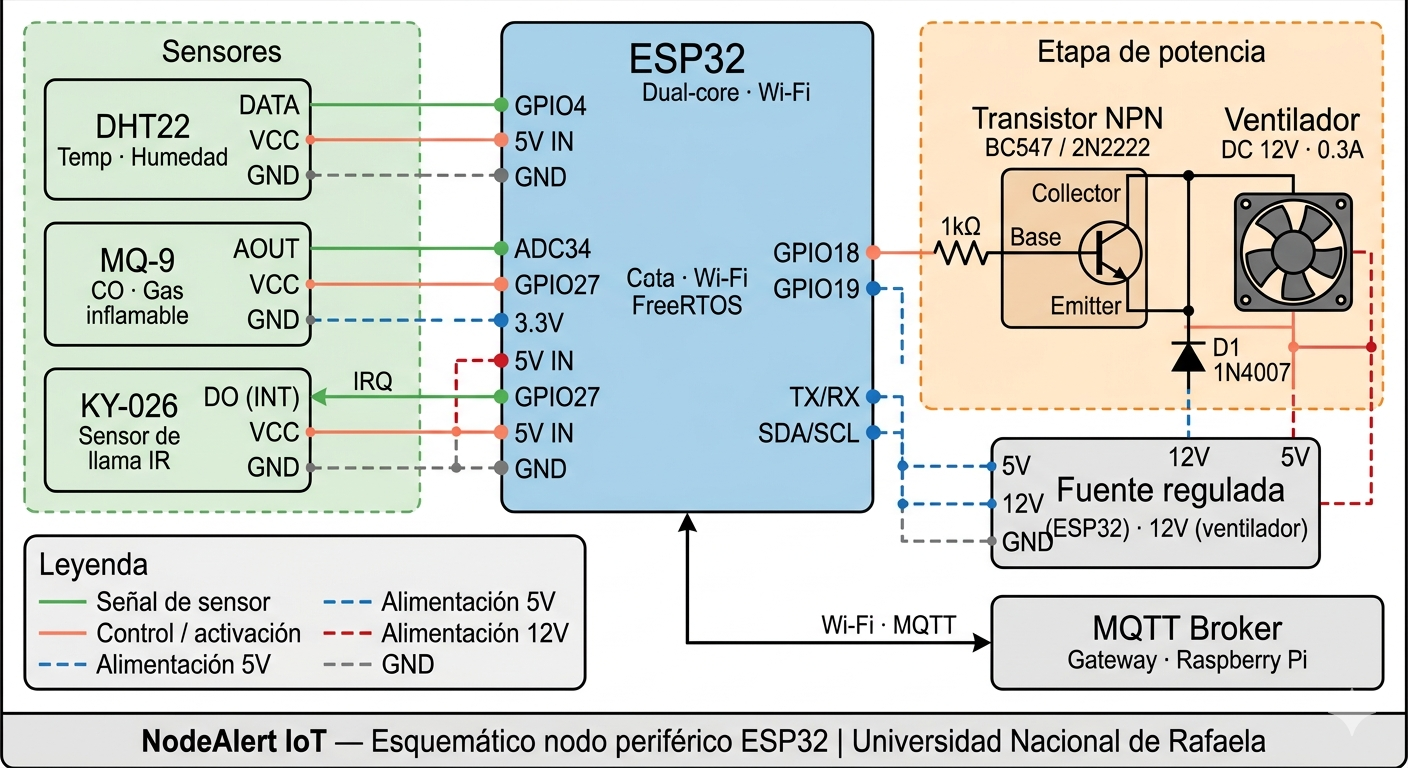
\includegraphics[width=0.9\linewidth]{esdd.png}
     \caption{Esquemático detallado del nodo periférico: Conexiones de sensores y etapa de potencia para el buzzer.}
    \label{fig:esquematico_hard}
 \end{figure}

% FOTO REAL: esdd.png